
\documentclass{beamer}
\usetheme{CambridgeUS}
\setbeamertemplate{blocks}[rounded][shadow=true]

% Color settings
\setbeamercolor{title}{bg=red!65!black, fg=white}

\setbeamercolor{block title}{use=structure,fg=white,bg=red!65!black}
\setbeamercolor{block body}{use=structure,fg=black,bg=black!3}

\setbeamercolor*{block title example}{fg=blue!50!black,bg=blue!10!white}
\setbeamercolor*{block body example}{fg=black,bg=blue!2}

% Margin
\setbeamersize{text margin left=30pt,text margin right=30pt}

\graphicspath{ {bilder/} }

% \AtBeginSection[]{%
% 	\begin{frame}
% 		\tableofcontents[currentsection]
% 	\end{frame}
% }% AtBeginSection

\AtBeginSubsection[]{%
\begin{frame}
\tableofcontents[currentsubsection]
\end{frame}
}% AtBeginSection

\mode<presentation>
{
\setbeamercovered{transparent}
}
\usepackage{amsmath,amsfonts,amssymb}
\usepackage[center]{caption}
\usepackage[utf8]{inputenc}
\usepackage[ngerman]{babel}
\usepackage{graphicx}
\usepackage{svg}
\usepackage{pdfpages}
\usepackage{placeins}
\usepackage[decimalsymbol=comma]{siunitx}

\usepackage{svg}
\usepackage{changepage}

\usepackage{mathptmx}
\usepackage[scaled=.90]{helvet}
\usepackage{courier}
\beamertemplatenavigationsymbolsempty 
\setbeamertemplate{footline}{}

%\usepackage[T1]{fontenc}
\title{Spurdetektoren}
\author[V. Grimm]{Verena Grimm}


\institute[]{
Seminarvortrag\\
Fachbereich Physik, Mathematik und Informatik (FB 08)\\
Johannes Gutenberg-Universität Mainz
}

\date{04.11.2014}


% Logo Universität
\titlegraphic{
\includegraphics[width=4cm]{bilder/JGU-Logo_sw_high.jpg}\hspace*{-8.5cm}}




\begin{document}

\begin{frame}
\titlepage
\end{frame}

\begin{frame}
\frametitle{Inhalt}
\tableofcontents
\end{frame}


%___________________________________________________________________________________________________
%___________________________________________________________________________________________________
%___________________________________________________________________________________________________

\section{Einführung}

\subsection[]{}
%___________________________________________________________________________________________________

\begin{frame}{Teilchendetektoren}
	\begin{description}
	  \item[Teilchendetektoren] Dienen dem Nachweis freier Teilchen durch Messung
	  verschiedener Parameter
	\end{description}
	
	\begin{block}{Häufig gemessene Eigenschaften}
		\begin{itemize}\setlength{\itemsep}{+5pt}
		  \item Geschwindigkeit
		  \item Impuls
		  \item Energie
		  \item Trajektorie
		  \item Zeit (Synchronisierung mit anderen Detektoren)
		  \item Ladung
		\end{itemize}
	\end{block}
\end{frame}

%___________________________________________________________________________________________________

	\begin{frame}{Spurdetektoren}
	\begin{description}
	  \item[Spurdetektoren] Bestimmen die Trajektorie eines Teilchens durch
	  Detektion an verschiedenen Orten und anschließender Rekonstruktion der
	  Bahnkurve
	\end{description}
	\begin{block}{Wozu die Trajektorie bestimmen?}
		\begin{itemize}\setlength{\itemsep}{+5pt}
		  \item Ursprung des Teilchens zurückverfolgen
		  	\begin{itemize}\setlength{\itemsep}{+5pt}
		    	\item Stammt Teilchen vom
		    	Kollisionspunkt$\rightarrow$Untergrundunterdrückung
		  	\end{itemize}
		  	\item \includesvg[svgpath=bilder/, width=5.7cm]{zerfallsstrecke}
		  	\item Messungen in Kombination mit Magnetfeld:
		   		\begin{itemize}\setlength{\itemsep}{+5pt}
		    		\item Ladung
		    		\item Impuls
		  		\end{itemize}
		\end{itemize}
	\end{block}
\end{frame}

\begin{frame}{Lorentzkraft}
	\begin{block}{Kraft auf geladene Teilchen bei magnetischer Flussdichte
	$\vec{B}$}
		$\vec{F}_L = q \cdot (\vec{v} \times \vec{B})$
	\end{block}
	\begin{block}{$\vec{F}_L$ führt zu Kreisbahn mit radius $r$}
		\begin{itemize}\setlength{\itemsep}{+5pt}
		  \item $r = \frac{m \cdot v}{q \cdot B} \propto \frac{p}{q}$
		  \item Vorzeichen der Krümmung ergibt Vorzeichen der Ladung $q$
		\end{itemize}
	\end{block}
	\begin{exampleblock}{Häufig ist Ladung erlaubter Sekundärteilchen eingeschränkt}
		$q \in \{- e, 0, +e\}$
		$\Rightarrow p = \pm e \cdot r \cdot B$
	\end{exampleblock}
\end{frame}
%___________________________________________________________________________________________________
%___________________________________________________________________________________________________

\subsection[]{}

%___________________________________________________________________________________________________

\begin{frame}{Pile-Up}
	An LHC-Experimenten wie ATLAS werden zukünftig alle 25 ns ca. 50
	Proton-Proton-Kollisionen gleichzeitig gemessen
	% http://iopscience.iop.org/1742-6596/513/2/022024/pdf/1742-6596_513_2_022024.pdf
	\begin{figure}[htp]
	\begin{center}
	  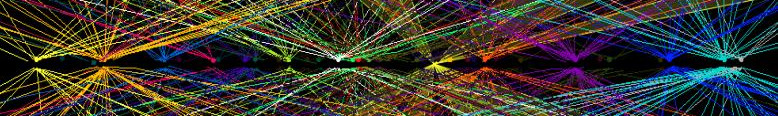
\includegraphics[width=\textwidth]{pileup.jpg}
	  \caption{Simulierter Pile-Up am CMS Detektor [cpu]}
	\end{center}
	\end{figure}
	\vspace{-0.7cm}
	\begin{block}{Jede Kollision muss isoliert analysiert werden (E- und
	p-Erhaltung)} Sekundärteilchen müssen je einer p-p-Kollision zugewiesen werden 
	\end{block}
	\begin{exampleblock}{Spurrekonstruktion nahe der Kollision}
		Schnittpunkt zwischen rekonstruierter Spur und Strahl stellt Ort der Kollision
		dar
	\end{exampleblock}
\end{frame}

%___________________________________________________________________________________________________




\subsection[]{Definition \& Grundlagen}




%___________________________________________________________________________________________________

\begin{frame}{Energieverlust in Materie}
	\begin{block}{Teilchendetektion $\Leftrightarrow$ Energieverlust im Detektor}
		Geladene und ungeladene Teilchen übertragen einen Teil ihrer Energie an die
		durchdrungene Materie	
	\end{block}
	
	
	% http://qgp.uni-muenster.de/~jowessel/pages/teaching/ss03/seminar/reiter.pdf
	\begin{block}{Viele verschiedene mögliche Mechanismen}
		\begin{itemize}
		  \item Bethe-Bloch-Formel
		  \item Rutherford-Streuung
		  \item Tscherenkow-Strahlung
		  \item Bremsstrahlung
		  \item Photoelektrischer Effekt
		  \item Compton-Streuung
		  \item Paarbildung
		  \item \ldots
		\end{itemize}
	\end{block}
\end{frame}

%___________________________________________________________________________________________________

\begin{frame}{Spurdetektoren}
	\begin{block}{Ziel von Teilchendetektoren}
		Absorbierte Energie in auswertbares Signal umwandeln 
	\end{block}
% 	\vspace{1cm}
	\begin{block}{Ziel der Spurdetektoren}
		Signal muss Ortsinformation beinhalten
	\end{block}
	
	\begin{exampleblock}{Idealer Spurdetektor}
		\begin{itemize}
		  \item möglichst wenig Masse (Vermeidung Vielfachstreuung/wenig Energieverlust)
		  \item gute Ortsauflösung
		  \item gute Zeitauflösung/geringe Totzeit
		  \item flexibel
		  \item günstig 
		\end{itemize}
	\end{exampleblock}
\end{frame}



%___________________________________________________________________________________________________
%___________________________________________________________________________________________________
%___________________________________________________________________________________________________

% \section{Grundlagen}


%___________________________________________________________________________________________________
%___________________________________________________________________________________________________
%___________________________________________________________________________________________________

\section{Gasdetektoren}
\subsection{Grundlagen}

\begin{frame}{Grundlagen}
	\begin{block}{Reaktionen von Strahlung mit Gasmolekülen}
		\begin{itemize}
		  \item Anregung:	$X+p\rightarrow X^*+p$\\
		  \item Ionisation:	$X+p\rightarrow X^++p+e^-$\\
		\end{itemize}		
	\end{block}

	\begin{block}{Arten der Ionisation}
		\begin{itemize}
		  \item primäre Ionisation: $e^-$/Ionen-Paare erzeugt durch eintreffende Strahlung
		  \item sekundäre Ionisation: freie $e^-$, die weitere $e^-$/Ionen-Paare erzeugen
		  etc.
		\end{itemize}
	\end{block}	
	
	\begin{block}{Warum Gas zum Teilchennachweis?}
		 hohe Mobilität der durch eintreffende Strahlung erzeugten Ionen und Elektronen
	\end{block}
\end{frame}


\begin{frame}{Grundlagen}
	\begin{block}{Mittlere Energie für Ionisation}
		\begin{itemize}
		  \item Energie, um $e^-$/Ionen-Paar zu erzeugen: ca. 30 eV
		  \item kaum abhängig von Teilchentyp und Gas
		\end{itemize}
	\end{block}
	\vspace*{0.7cm}
	Um $e^-$/Ionen-Paare zu sammeln, müssen beide lange genug frei sein
	\begin{block}{Hindernisse}
			\begin{itemize}
		  \item Rekombination unter Aussendung eines Photons
		  \item Elektronenbindung: Einfangen freier $e^-$ durch elektrogenative Atome unter Aussendung
		  eines Photons
		\end{itemize}
	\end{block}
\end{frame}

\begin{frame}{Transport}
	\begin{block}{Diffusion}
	\begin{itemize}
		  \item ohne $E$-Feld: $e^-$/Ionen-Paare diffundieren vom Ort des Entstehens weg $\rightarrow$
		  Verlust an Energie durch Zusammenstöße $\rightarrow$ therm. Gleichgewicht $\rightarrow$
		  Rekombination
		  \item Geschwindigkeit im therm. Gleichgewicht: Maxwell-Verteilung\\
		  		$v=\sqrt{\frac{8kT}{\pi m}}$
% 		  \item Diffusionskoeffizient: $D=\frac{1}{3}\cdot v\cdot \lambda$
% 		 		$\rightarrow$ je höher $D$, desto höher die Ausbreitung pro Zeit $t$
		\end{itemize}
	\end{block}
	
	\begin{block}{Drift}
	\begin{itemize}
		  \item mit $E$-Feld: $e^-$/Ionen-Paare beschleunigen entlang der Feldlinien
		  \item Beschleunigung unterbrochen durch Kollisionen mit Gasmolekülen\\
		  		$\rightarrow$ Geschwindigkeitszunahme begrenzt!
		  \item mittlere Geschw.: \bf{Driftgeschwindigkeit $u$}
		  \item $u=\mu E$~~~mit~~~$\mu=\frac{D\cdot e}{kT}$ 
		\end{itemize}
	\end{block}
\end{frame}


\subsection[]{Nebel- und Blasenkammer}

%___________________________________________________________________________________________________

\begin{frame}{Nebelkammer}
	Erfindung 1911 durch Charles Wilson
	\vspace{0.7cm}
	\begin{block}{Kammer mit übersättigtem Wasserdampf}
		\begin{itemize}
		  \item Ionisierende Strahlung bildet Ionen-Elektronen-Paare im Gas
		  \item Ionen wirken als Kondensationskeim
		  \item Kondensierte Tröpfchen bilden sichtbaren Kondensstreifen 
		  \item Fotografie der Kondensstreifen für spätere Spurrekonstruktion
		\end{itemize}
	\end{block}
	\vspace{0.7cm}
	Später: Übersättigte Luft-Alkohol-Gemische\\

\end{frame}

%___________________________________________________________________________________________________



\begin{frame}{Funkenkammer - Aufbau}
    \begin{columns}[T]
    
	    \column{.5\textwidth}
			\begin{figure}[htbp]
			  \centering
			  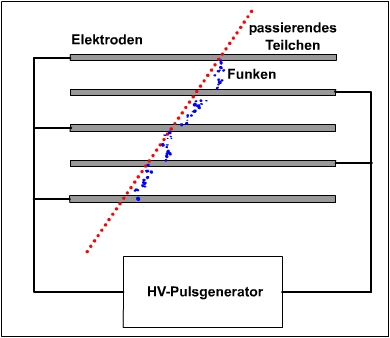
\includegraphics[width=\textwidth]{prinzipfk.jpg}
			  \caption{Aufbau einer Funkenkammer [gfa]}
			\end{figure}
			
	    \column{.5\textwidth}
	    	\begin{itemize}
			  \item Zwischen mehreren leitenden Platten in Edelgas liegt abwechselnde HV an
			  \item Ionisierende Strahlung bildet Ionen-Elektronen-Paare im Gas
			  \item Funken springen zwischen Platten über - entlang der Ionisationsspur
			  \item HV meist getriggert durch Szintillatoren
			\end{itemize}
    \end{columns}
\end{frame}

%___________________________________________________________________________________________________

\begin{frame}{Nebel- und Funkenkammer}
    \begin{columns}[T]
	    \column{.5\textwidth}
	    \center{Nebelkammer [gnk]}
			\begin{figure}[htbp]
			  \centering
			  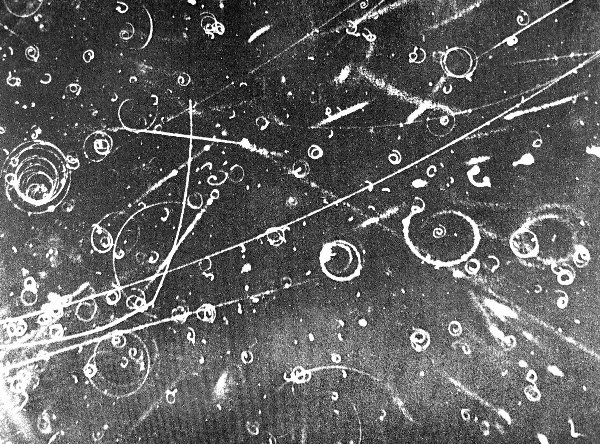
\includegraphics[width=\columnwidth]{nebelkammer.jpg}
			\end{figure}
			
	    \column{.5\textwidth}
	    \center{Funkenkammer [gfk]}
	    	\begin{figure}[htbp]
			  \centering
			  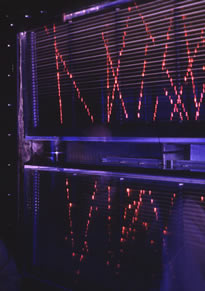
\includegraphics[width=\columnwidth*2/3]{funkenkammer.jpg}
			\end{figure}
    \end{columns}
\end{frame}

\begin{frame}{Nebel- und Funkenkammer}
	    \center{Entdeckung des Positrons (1932) [epo]}
			\begin{figure}[htbp]
			  \centering
			  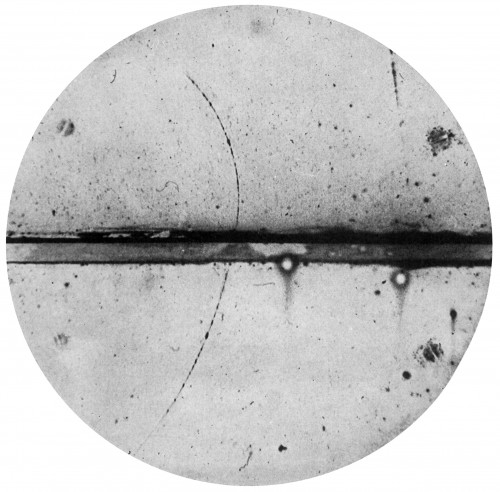
\includegraphics[scale=0.3]{positron.jpg}
			\end{figure}
		Weiterhin: Nachweis Comptoneffekt, Paarerzeugung/-vernichtung, \ldots
\end{frame}

% \begin{frame}{Blasenkammer}
% 	Erfindung 1952 durch Donals A. Glaser
% 	\begin{block}{Ähnliches Prinzip wie Nebelkammer}
% 		\begin{itemize}
% 		  \item Metastabiler Zustand von flüssigem Wasserstoff bei adiabatischer
% 		  Druckänderung
% 		  \item Ionen wirken als Siedekeim
% 		  \item Entstandene Bläschen visualisieren Teilchenspur 
% 		  \item Fotografie der Blasenspuren für spätere Rekonstruktion
% 		\end{itemize}
% 	\end{block}
% \end{frame}
% 
% %___________________________________________________________________________________________________
% 
% \begin{frame}{Blasenkammer - Aufbau}
%     \begin{columns}[T]
%     
% 	    \column{.6\textwidth}
% 			\begin{figure}[htbp]
% 			  \centering
% 			  \includesvg[svgpath=bilder/, width=\textwidth]{Blasenkammer}
% 			  \caption{Blasenkammer mit B-Feld [wbk]}
% 			\end{figure}
% 			
% 	    \column{.45\textwidth}
% 	    	\begin{enumerate}
% 			  \item Kurz vor Messung wird Druck verringert
% 			  \item Temperatur nun oberhalb des Siedepunktes
% 			  \item Kameras bilden Blasenspuren ab
% 			  \item 3D-Rekonstruktion der Spuren möglich
% 			  \item Druck wird wieder erhöht damit sich Blasen wieder lösen  
% 			\end{enumerate}
%     \end{columns}
% \end{frame}

%___________________________________________________________________________________________________

\begin{frame}{Nebel- und Funkenkammern}
    \begin{columns}[T]
		\column{.45\textwidth}
			\textbf{Vorteile}		
			\vspace{0.7cm}
			\begin{itemize}
			  \item Bahnen direkt sichtbar (einfache Rekonstruktion)
			  \item Günstig
			  \item Voller Raumwinkel bei Nebelkammer
			\end{itemize}	
	    \column{.5\textwidth}
	    	\textbf{Nachteile}
	    	\vspace{0.7cm}
	    	\begin{itemize}
			  \item Langsame Bildung der Spur (Nebelkammer)
			  \item Nur Nebelkammer kann kontinuierlich betrieben werden
			  \item Viel Materie (WW mit Teilchen)
			  \item Ortsauflösung Funkenkammer: $O(1 mm)$
			\end{itemize}
    \end{columns}
    \vspace{1cm}
    Heute: Nur noch für demonstrative Zwecke
\end{frame}
\subsection[]{Zählrohr}

\begin{frame}{Zählrohr}
    \begin{columns}[T]
    
	    \column{.6\textwidth}
			\begin{figure}[htbp]
			  \centering
			  \includesvg[svgpath=bilder/, width=\textwidth]{zaehlrohr}
			  \caption{Aufbau eines Zählrors [wzr]}
			\end{figure}
			
	    \column{.45\textwidth}
	    	\begin{itemize}
	    	  \item Gasgefülltes Rohr
			  \item Hochspannung zwischen Kathode und Anode
			  \item Ionisierende Strahlung bildet freie Elektronen
			  \item Diese driften zur Anode	
			  \item Stromimpuls wird gemessen
			\end{itemize}
    \end{columns}
\end{frame}

%___________________________________________________________________________________________________

\begin{frame}{Zählrohr-Kennlinie}
	Zählrohrspannung beschleunigt freie Elektronen Richtung Anode \\
	Funktionsweise stark abhängig von Spannung
	
	\begin{figure}[htbp]
	  \centering
	  \includesvg[svgpath=bilder/, height=0.5\textheight]{zaehlrohr-kennlinie}
	  \caption{Kennlinie eines Zählrors [wzk]}
	\end{figure}
	
\end{frame}	

%___________________________________________________________________________________________________

\begin{frame}{Zählrohr-Modi}
	\begin{block}{Geringe Spannung ($\ll 100V$): Rekombination}
		\begin{itemize}
		  	\item $e^-$ können mit Ionen rekombinieren
		  	\item Nur wenige Elektronen erreichen Anode
		  	\item Strompuls abhängig von Abstand der Ionisation
		\end{itemize}
	\end{block}
	
	\begin{block}{Höhere Spannung ($O(100V)$): Ionisationskammer}
		\begin{itemize}
		  	\item Keine Rekombination: Alle $e^-$ erreichen Anode
		  	\item Strompuls proportional zur Anzahl der Elektronen
			\item \textbf{Messung der absorbierten Energie möglich}
		\end{itemize}
	\end{block}
	
\end{frame}

\begin{frame}{Zählrohr-Modi}
	\begin{block}{Höhere Spannung: Proportionalzählrohr}
		\begin{itemize}
		  	\item $e^-$ ionisieren nahe der Anode weitere Atome (Lawinen)
			\item $\Rightarrow$ Verstärkung des Strompulses
		  	\item Signal weiterhin proportional zur absorbierten Energie
		\end{itemize}
	\end{block}
	
	\begin{block}{Höchste Spannung: Geiger-Müller-Bereich}
		\begin{itemize}
	  		\item Energie so hoch, dass UV-Strahlung entsteht, die weitere Stellen
	  		Ionisiert
	  		\item Komplette Ionisierung der Kammer $\Rightarrow$ Gasentladung
	  		\item Keine Energiemessung $\Leftrightarrow$ Reiner Zähler
	  		\item Hohe Totzeit (ca. $100\mu s$)
		\end{itemize}
	\end{block}
	Noch höhere Spannung führt zur spontanen Gasentladung
\end{frame}

\subsection[]{Vieldrahtproportionalkammer}


\begin{frame}{Vieldrahtproportionalkammer oder MWPC}
    \begin{columns}[T]
	    \column{.5\textwidth}
			\begin{figure}[htbp]
			  \centering
			  \includesvg[svgpath=bilder/, width=\textwidth]{vieldraht}
			  \caption{Aufbau einer Vieldrahtkammer [wvk]}
			\end{figure}
			
	    \column{.45\textwidth}
	    	\begin{itemize}
	    	  \item Proportionalkammer mit vielen Drähten statt einem
			  \item äquidistante Drähte (Anode) zwischen zwei Platten (Kathode)
			\end{itemize}
			
			\begin{figure}[htbp]
			  \centering
			  \includesvg[svgpath=bilder/, width=\columnwidth*2/3]{vieldrahtfeld}
			  \caption{Feldlinien einer Vieldrahtkammer [wvkf]}
			\end{figure}
    \end{columns}
\end{frame}



\begin{frame}{Vieldrahtproportionalkammer}
    	\begin{block}{Wie kommt die Spur zustande?}
		\begin{itemize}
		  \item $e^-$/Ionen-Paare driften entlang der Feldlinien zur nächsten Anode/Kathode
		  \item $e^-$ lösen bei hoher Feldliniendichte Ladungslawine an Anode aus $\rightarrow$
		  Signal$\rightarrow$ eindimensionale Ortsauflösung
		  \item 2D: zweite Lage von Drähten senkrecht auf erster ($X-Y$ MWPC)
		  \item 3D: mehrere MWPC hintereinander
		\end{itemize}
	\end{block}
\end{frame}

\begin{frame}{Vieldrahtproportionalkammer}
    \begin{columns}[T]
		\column{.45\textwidth}
			\textbf{Vorteile}	
			\vspace{0.7cm}	
			\begin{itemize}
				\item einfacher Aufbau
			  	\item Energiemessung möglich
			  	\item elektronische Auslese leicht möglich
			  	\item geringe Totzeit 
			\end{itemize}	
	    \column{.5\textwidth}
	    	\textbf{Nachteile}
	    	\vspace{0.7cm}
	    	\begin{itemize}
			  \item schlechte Ortsauflösung ($O(mm)$)
			  \item viele Kanäle
			\end{itemize}
    \end{columns}
    \vspace{1cm}
\end{frame}

\begin{frame}{Vieldrahtproportionalkammer}
    Beispielbild?
\end{frame}

\subsection[]{Driftkammer}

\begin{frame}{Driftkammer}
    \begin{columns}[T]
	    \column{.5\textwidth}
			\begin{figure}[htbp]
			  \centering
			  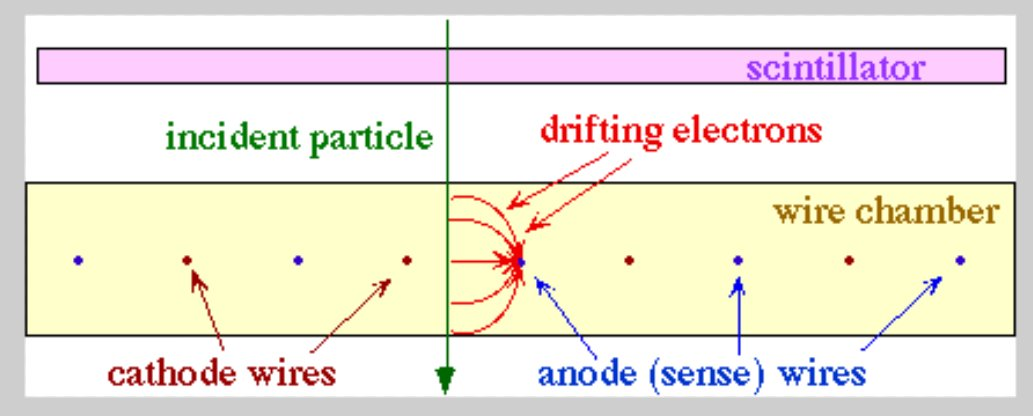
\includegraphics[width=\textwidth]{drift.jpg}
			  \caption{Aufbau einer Driftkammer}
			\end{figure}
			
	    \column{.55\textwidth}
	    	\begin{itemize}
	    	  \item Messung der Ortsinformation durch Messung der Driftzeit
			  \item Aufbau: Proportionalzähler mit Trigger (Szintillator $\rightarrow$ schnelles Signal)
			  \item Trigger gibt den Zeitpunkt $t_0$, an dem Teilchen eintrifft
			  \item Anode gibt den Zeitpunkt $t_1$, an dem Signal (Elektronen) eintrifft
			  \item bei bekannter Driftgeschw. $u$: Distanz von Enstehungsort zu Anode ist
			  $x=\int_{t_0}^{t_1}u\cdot dt$
			\end{itemize}
			
    \end{columns}
\end{frame}

\begin{frame}{Driftkammer}

	\begin{block}{Wie kommt die Spur zustande?}
		\begin{itemize}
		  \item mehrere Ebenen hintereinander, um Spur zu rekonstruieren
		  \item verschiedene Orientierungen der Drähte
		\end{itemize}
	\end{block}
	\vspace{0.8cm}
    \begin{columns}[T]
		\column{.45\textwidth}
			Vorteile		
			\begin{itemize}
			  \item großflächiger Aufbau möglich
			  \item wenige Kanäle
			  \item gute Ortsauflösung ($O(100\mu m)$)
			\end{itemize}	
	    \column{.5\textwidth}
	    	Nachteile
	    	\begin{itemize}
			  \item Größerer Abstand der Drähte $\rightarrow$ höhere Rate pro Draht 
			\end{itemize}
    \end{columns}
    \vspace{1cm}
\end{frame}

\begin{frame}{Driftkammer}
    Beispielbild?
\end{frame}
% \input{tpc}
% \input{gems}
% \input{micromegas}

%___________________________________________________________________________________________________
%___________________________________________________________________________________________________
%___________________________________________________________________________________________________


% \section{Halbleiterdetektoren}
% \input{Pixeldetektoren}
% \input{nummer2}
% \input{nummer3?}

%___________________________________________________________________________________________________
%___________________________________________________________________________________________________

\section{Pixeldetektoren}

%___________________________________________________________________________________________________
%___________________________________________________________________________________________________
%___________________________________________________________________________________________________

\section{Spurrekonstruktion}

%___________________________________________________________________________________________________
%___________________________________________________________________________________________________

\subsection{Hough-Transformation}


%___________________________________________________________________________________________________

\begin{frame}{Literaturverzeichnis}
	\begin{adjustwidth}{-5em}{-2em}
	  	\begin{description}
		  	\item[wbk]
		  	https://de.wikipedia.org/w/index.php?title=Datei:Blasenkammer.svg
		  	\item[wzr]
		  	https://de.wikipedia.org/wiki/Datei:Geiger\_Mueller\_Counter\_with\_Circuit-de.svg
		  	\item[wzk]
			http://de.wikipedia.org/wiki/Datei:Kennlinie\_Zaehlrohr-GER.svg
			\item[wvk]
		  	http://de.wikipedia.org/wiki/Drahtkammer\#mediaviewer/File:Wire\_ chamber\_schematic.svg
		  	\item[wvkf]
		  	http://upload.wikimedia.org/wikipedia/commons/2/22/Wire\_chamber\_E\_field.svg
		  	\item[cpu]
		  	http://francis.naukas.com/2012/06/16/ya-hay-colisiones-proton-proton-en-el-lhc-que-presentan-mas-de-30-vertices-apilados/
		\end{description}
	\end{adjustwidth}  
\end{frame}

\end{document}